% ══════════════════════════════════════════════════════════════
%  Ensemble Learning for Telecom Customer Churn Prediction
%  Beamer Presentation — Defense
%  Compiler: pdfLaTeX
% ══════════════════════════════════════════════════════════════
\documentclass[aspectratio=169,11pt]{beamer}

% ── Theme: clean, peaceful, serious ──
\usetheme{default}
\usecolortheme{seahorse}
\usefonttheme{professionalfonts}

\setbeamertemplate{navigation symbols}{}
\setbeamertemplate{footline}[frame number]
\setbeamertemplate{itemize items}[circle]
\setbeamertemplate{enumerate items}[default]

% Colors — calm blue-teal palette
\definecolor{mainblue}{HTML}{1e3a5f}
\definecolor{accentteal}{HTML}{2d8a7e}
\definecolor{softgray}{HTML}{f0f4f8}
\definecolor{warmwhite}{HTML}{fafbfc}
\definecolor{subtletext}{HTML}{5a6e82}
\definecolor{dangerred}{HTML}{c0392b}
\definecolor{successgreen}{HTML}{27ae60}

\setbeamercolor{title}{fg=mainblue}
\setbeamercolor{frametitle}{fg=mainblue,bg=softgray}
\setbeamercolor{structure}{fg=accentteal}
\setbeamercolor{normal text}{fg=mainblue}
\setbeamercolor{block title}{fg=white,bg=accentteal}
\setbeamercolor{block body}{bg=softgray}
\setbeamercolor{block title alerted}{fg=white,bg=dangerred}
\setbeamercolor{block body alerted}{bg=softgray}
\setbeamercolor{block title example}{fg=white,bg=successgreen}
\setbeamercolor{block body example}{bg=softgray}

\setbeamerfont{title}{size=\Large,series=\bfseries}
\setbeamerfont{frametitle}{size=\large,series=\bfseries}

% ── Packages ──
\usepackage[utf8]{inputenc}
\usepackage[T1]{fontenc}
\usepackage{lmodern}
\usepackage{graphicx}
\usepackage{booktabs}
\usepackage{amsmath,amssymb}
\usepackage{tikz}
\usepackage{pgfplots}
\pgfplotsset{compat=1.18}
\usetikzlibrary{shapes.geometric,arrows.meta,positioning,calc,decorations.pathreplacing,fit,backgrounds}
\usepackage{multicol}
\usepackage{xcolor}
\usepackage{fontawesome5}
\usepackage{adjustbox}
\usepackage{hyperref}

\hypersetup{colorlinks=false}

\graphicspath{{reports/}}

% Shortcut commands
\newcommand{\emphasis}[1]{\textcolor{accentteal}{\textbf{#1}}}
\newcommand{\metricbox}[2]{%
  \begin{tikzpicture}
    \node[rounded corners=4pt, fill=softgray, minimum width=2.2cm, minimum height=1.1cm, align=center] {
      {\scriptsize\color{subtletext}#1}\\[2pt]
      {\large\bfseries\color{mainblue}#2}
    };
  \end{tikzpicture}%
}

% ══════════════════════════════════════════════════════════════
\title{Ensemble Learning for\\Customer Churn Prediction}
\subtitle{A Diversity-Driven Approach with Business Decision Support}
\author{Zaynab Raounak}
\date{April 2025}

\begin{document}

% ── TITLE ──
\begin{frame}[plain]
  \begin{tikzpicture}[remember picture,overlay]
    \fill[mainblue] (current page.north west) rectangle (current page.south east);
    \fill[accentteal,opacity=0.15] (current page.north west) rectangle (current page.south east);
    % Subtle decorative circles
    \fill[white,opacity=0.03] (12,2) circle (4);
    \fill[white,opacity=0.03] (-2,-1) circle (3);
    \fill[white,opacity=0.05] (14,-2) circle (2);
  \end{tikzpicture}
  \begin{tikzpicture}[remember picture,overlay]
    \node[anchor=center] at (current page.center) {
      \begin{minipage}{0.8\textwidth}
        \centering
        \color{white}
        {\Huge\bfseries Ensemble Learning for\\[6pt] Customer Churn Prediction}\\[16pt]
        {\large A Diversity-Driven Approach\\with Business Decision Support}\\[24pt]
        \rule{4cm}{0.4pt}\\[12pt]
        {\normalsize Zaynab Raounak}\\[4pt]
        {\small\color{white!70} April 2025}
      \end{minipage}
    };
  \end{tikzpicture}
\end{frame}

% ── OUTLINE ──
\begin{frame}{Outline}
  \begin{columns}[T]
    \column{0.5\textwidth}
    \begin{enumerate}
      \item[\faIcon{crosshairs}] Problem \& Motivation
      \item[\faIcon{database}] Data \& Feature Engineering
      \item[\faIcon{project-diagram}] Model Architecture
      \item[\faIcon{random}] Diversity Analysis
    \end{enumerate}
    \column{0.5\textwidth}
    \begin{enumerate}
      \setcounter{enumi}{4}
      \item[\faIcon{chart-bar}] Results \& Comparison
      \item[\faIcon{balance-scale}] Calibration \& Cost Optimization
      \item[\faIcon{desktop}] Web Platform Demo
      \item[\faIcon{flag-checkered}] Conclusion
    \end{enumerate}
  \end{columns}
\end{frame}

% ══════════════════════════════════════════════════════════════
%  1. PROBLEM & MOTIVATION
% ══════════════════════════════════════════════════════════════
\begin{frame}{The Churn Problem}
  \begin{columns}[c]
    \column{0.55\textwidth}
    \begin{itemize}
      \item Telecom industry: acquiring a new customer costs \emphasis{5--7$\times$} more than retaining one
      \item A company with 26\% churn loses \emphasis{millions annually} in lifetime revenue
      \item Early identification enables targeted interventions
    \end{itemize}
    \vspace{10pt}
    \begin{alertblock}{Research Question}
      Can \textbf{diversity-aware ensemble learning} outperform individual models and deliver reliable, cost-optimized predictions for business deployment?
    \end{alertblock}

    \column{0.42\textwidth}
    \centering
    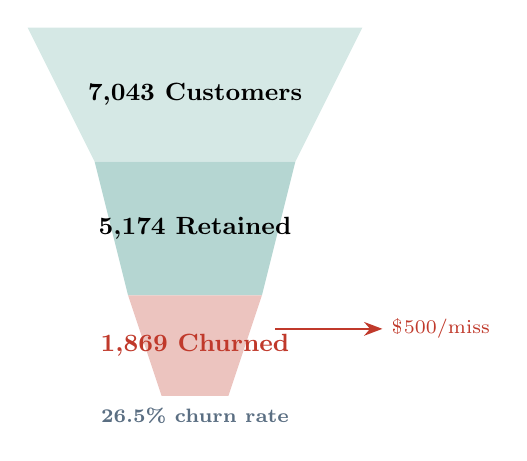
\begin{tikzpicture}[scale=0.85]
      % Funnel
      \fill[accentteal!20] (-2.5,4) -- (2.5,4) -- (1.5,2) -- (-1.5,2) -- cycle;
      \fill[accentteal!35] (-1.5,2) -- (1.5,2) -- (1,0) -- (-1,0) -- cycle;
      \fill[dangerred!30] (-1,0) -- (1,0) -- (0.5,-1.5) -- (-0.5,-1.5) -- cycle;
      \node at (0,3) {\small\bfseries 7,043 Customers};
      \node at (0,1) {\small\bfseries 5,174 Retained};
      \node[text=dangerred] at (0,-0.75) {\small\bfseries 1,869 Churned};
      \node[text=subtletext] at (0,-1.8) {\scriptsize\textbf{26.5\% churn rate}};
      % Arrow out
      \draw[-{Stealth},dangerred,thick] (1.2,-0.5) -- (2.8,-0.5) node[right,font=\scriptsize,text=dangerred] {\$500/miss};
    \end{tikzpicture}
  \end{columns}
\end{frame}

% ══════════════════════════════════════════════════════════════
%  2. DATA & FEATURE ENGINEERING
% ══════════════════════════════════════════════════════════════
\begin{frame}{Data \& Feature Engineering}
  \begin{columns}[T]
    \column{0.48\textwidth}
    \begin{block}{Dataset: Telco Customer Churn}
      \begin{itemize}
        \item 7,043 customers, 21 raw features
        \item Demographics, services, billing, contract
        \item Binary target: Churn (Yes/No)
        \item Train 70\% / Val 10\% / Test 20\%
      \end{itemize}
    \end{block}

    \column{0.48\textwidth}
    \begin{block}{9 Engineered Features}
      \begin{itemize}
        \item \texttt{AvgMonthlyCharge}
        \item \texttt{ChargeIncrease}
        \item \texttt{MonthlyToTotalRatio}
        \item \texttt{tenure\_bin} (4 segments)
        \item \texttt{IsNewCustomer} ($\leq$6 months)
        \item \texttt{NumServices}
        \item \texttt{HasSecurity}
        \item \texttt{HasSupport}
        \item \texttt{AutoPay}
      \end{itemize}
    \end{block}
  \end{columns}

  \vspace{8pt}
  \centering
  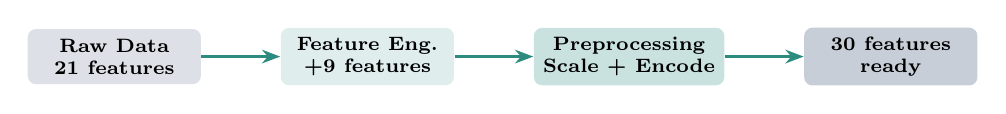
\begin{tikzpicture}[
    box/.style={rounded corners=3pt, minimum width=2.2cm, minimum height=0.7cm, align=center, font=\scriptsize\bfseries},
    arr/.style={-{Stealth}, thick, accentteal}
  ]
    \node[box, fill=mainblue!15] (raw) {Raw Data\\21 features};
    \node[box, fill=accentteal!15, right=1cm of raw] (feat) {Feature Eng.\\+9 features};
    \node[box, fill=accentteal!25, right=1cm of feat] (pre) {Preprocessing\\Scale + Encode};
    \node[box, fill=mainblue!25, right=1cm of pre] (train) {30 features\\ready};
    \draw[arr] (raw) -- (feat);
    \draw[arr] (feat) -- (pre);
    \draw[arr] (pre) -- (train);
  \end{tikzpicture}
\end{frame}

% ══════════════════════════════════════════════════════════════
%  3. MODEL ARCHITECTURE
% ══════════════════════════════════════════════════════════════
\begin{frame}{Model Architecture — 4 Learning Families}
  \centering
  \begin{tikzpicture}[
    family/.style={rounded corners=5pt, minimum width=3.2cm, minimum height=1.6cm, align=center, font=\small},
    meta/.style={rounded corners=5pt, minimum width=4cm, minimum height=1cm, align=center, font=\small\bfseries, fill=mainblue!20},
    arr/.style={-{Stealth}, thick, gray!50}
  ]
    % 4 families
    \node[family, fill=accentteal!15] (tree) at (0,2.5) {\textbf{Tree-Based}\\{\scriptsize RF, XGB, LGBM, GBM,}\\{\scriptsize AdaBoost, Bagging, ET}};
    \node[family, fill=blue!10] (linear) at (4.5,2.5) {\textbf{Linear}\\{\scriptsize Logistic}\\{\scriptsize Regression}};
    \node[family, fill=orange!10] (kernel) at (9,2.5) {\textbf{Kernel}\\{\scriptsize SVM}\\{\scriptsize (RBF)}};
    \node[family, fill=purple!10] (neural) at (13,2.5) {\textbf{Neural}\\{\scriptsize MLP}\\{\scriptsize (64-32)}};

    % Meta-ensembles
    \node[meta] (stack) at (3,-0.2) {\faIcon{layer-group}\ \ Stacking (6 base + LR meta)};
    \node[meta] (vsoft) at (8.5,-0.2) {\faIcon{wave-square}\ \ Soft Voting (6 models)};
    \node[meta] (vhard) at (13,-0.2) {\faIcon{vote-yea}\ \ Hard Voting (7 models)};

    % Arrows
    \draw[arr] (tree.south) -- ++(0,-0.4) -| (stack.north);
    \draw[arr] (linear.south) -- ++(0,-0.4) -| (stack.north);
    \draw[arr] (kernel.south) -- ++(0,-0.3) -| (vsoft.north);
    \draw[arr] (neural.south) -- ++(0,-0.3) -| (vsoft.north);
    \draw[arr] (tree.south) -- ++(0,-0.6) -| (vhard.north);

    % Label
    \node[font=\scriptsize, text=subtletext] at (8,-1.2) {Diverse families $\rightarrow$ complementary error patterns $\rightarrow$ stronger ensembles};
  \end{tikzpicture}
\end{frame}

% ══════════════════════════════════════════════════════════════
%  4. DIVERSITY ANALYSIS
% ══════════════════════════════════════════════════════════════
\begin{frame}{Why Diversity Matters}
  \begin{columns}[c]
    \column{0.52\textwidth}
    \begin{itemize}
      \item Ensembles only improve when members make \emphasis{different errors}
      \item Tree-only ensembles: Q-statistic $>$ 0.95 \\ {\small\color{dangerred} $\rightarrow$ nearly redundant}
      \item After adding LR, SVM, MLP: Q drops to \emphasis{0.663} \\ {\small\color{successgreen} $\rightarrow$ genuinely diverse}
    \end{itemize}
    \vspace{6pt}
    \begin{exampleblock}{Key Finding}
      The \textbf{maximally diverse subset} \{RF, LogReg\} achieves AUC = 0.863 with \textbf{only 2 models} --- matching the full 6-model stacking ensemble.
    \end{exampleblock}

    \column{0.46\textwidth}
    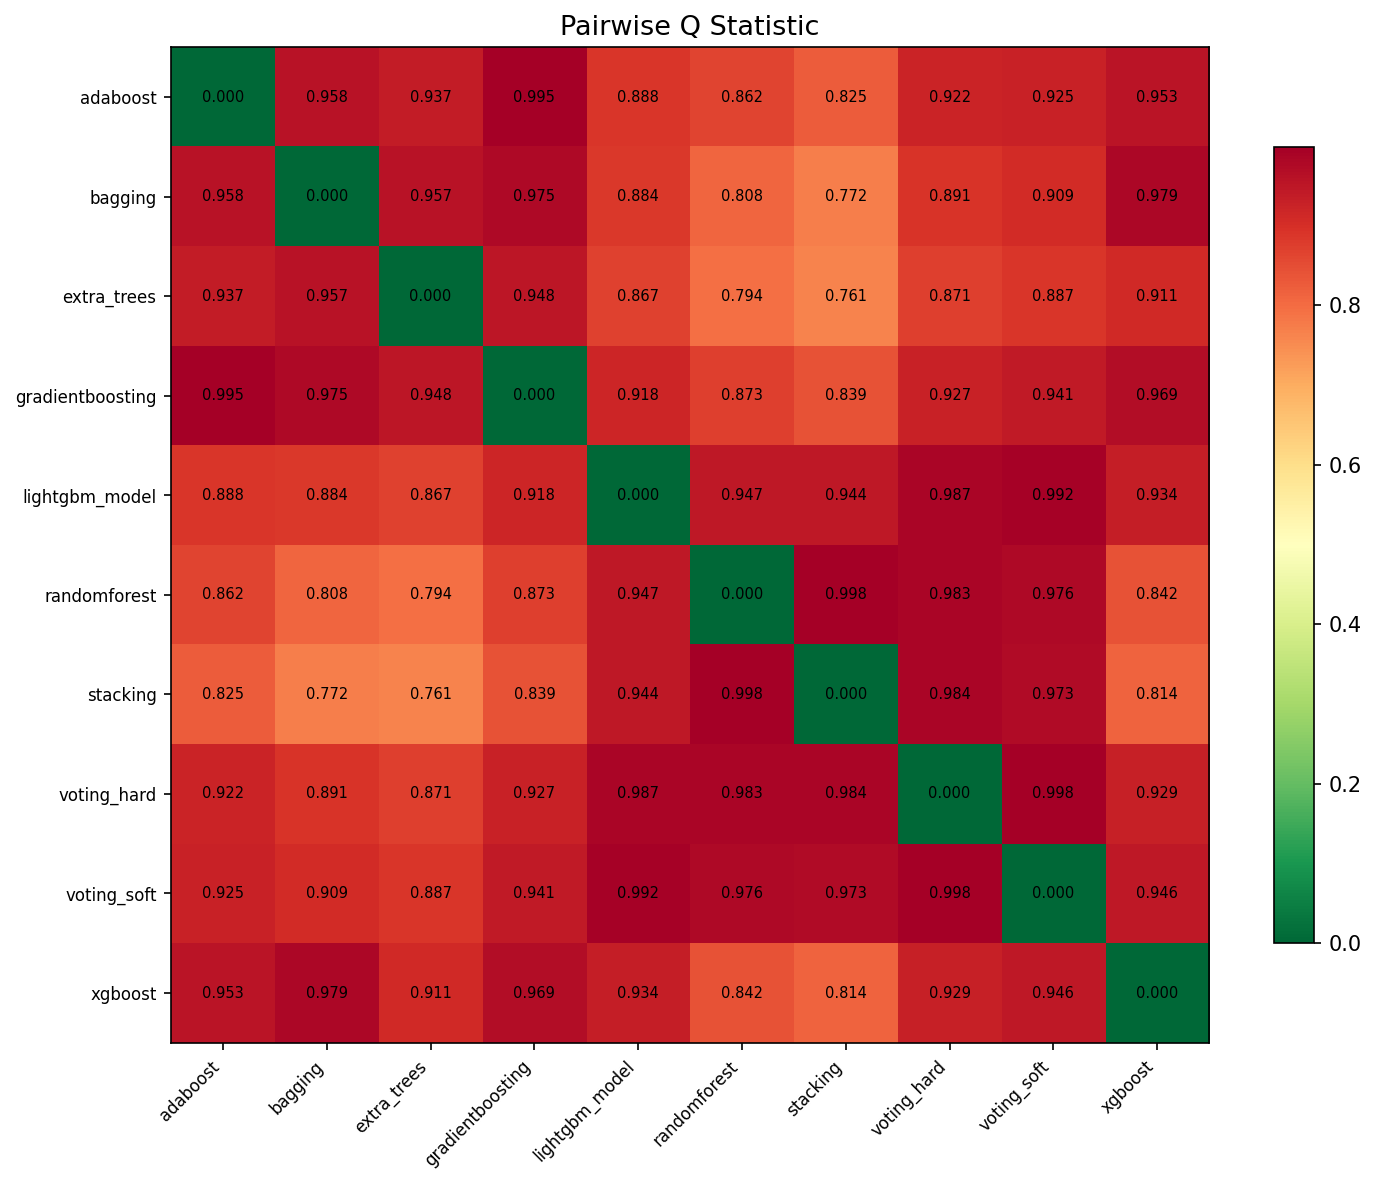
\includegraphics[width=\linewidth]{diversity_q_statistic.png}
    \vspace{-4pt}
    \centering{\scriptsize\color{subtletext} Q-Statistic Heatmap --- lower is more diverse}
  \end{columns}
\end{frame}

\begin{frame}{Diversity Metrics — Disagreement \& Double-Fault}
  \begin{columns}[c]
    \column{0.48\textwidth}
    \centering
    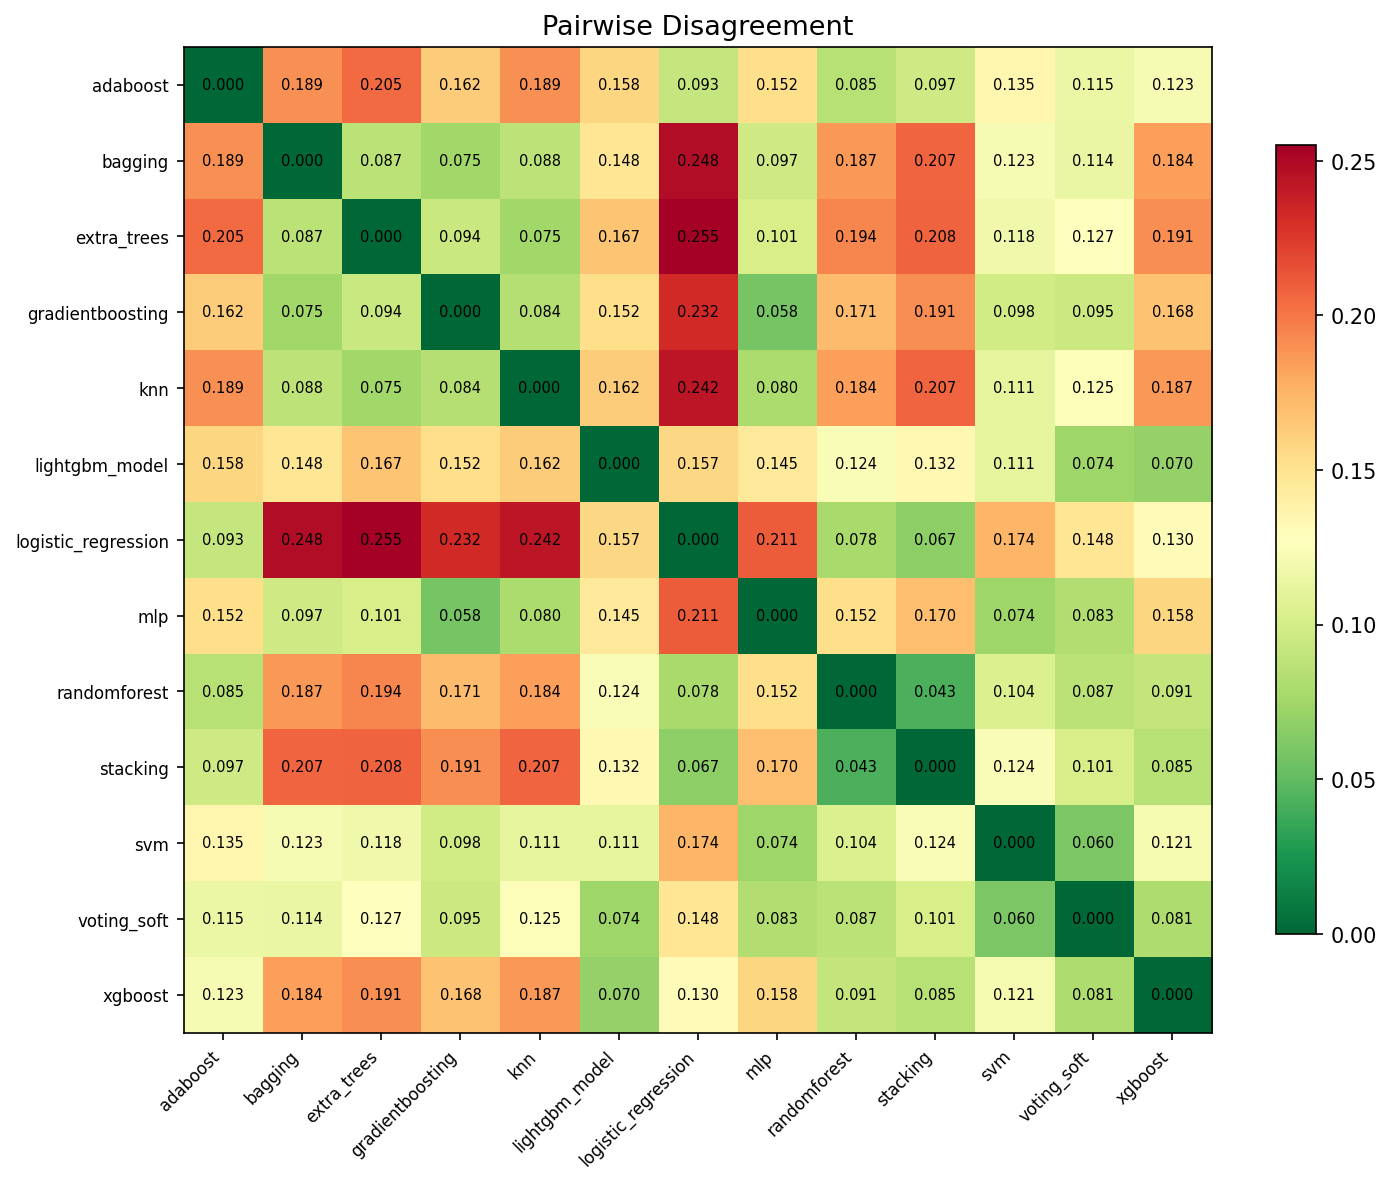
\includegraphics[width=\linewidth]{diversity_disagreement.png}
    {\scriptsize\color{subtletext} Disagreement rate (higher = more diverse)}

    \column{0.48\textwidth}
    \centering
    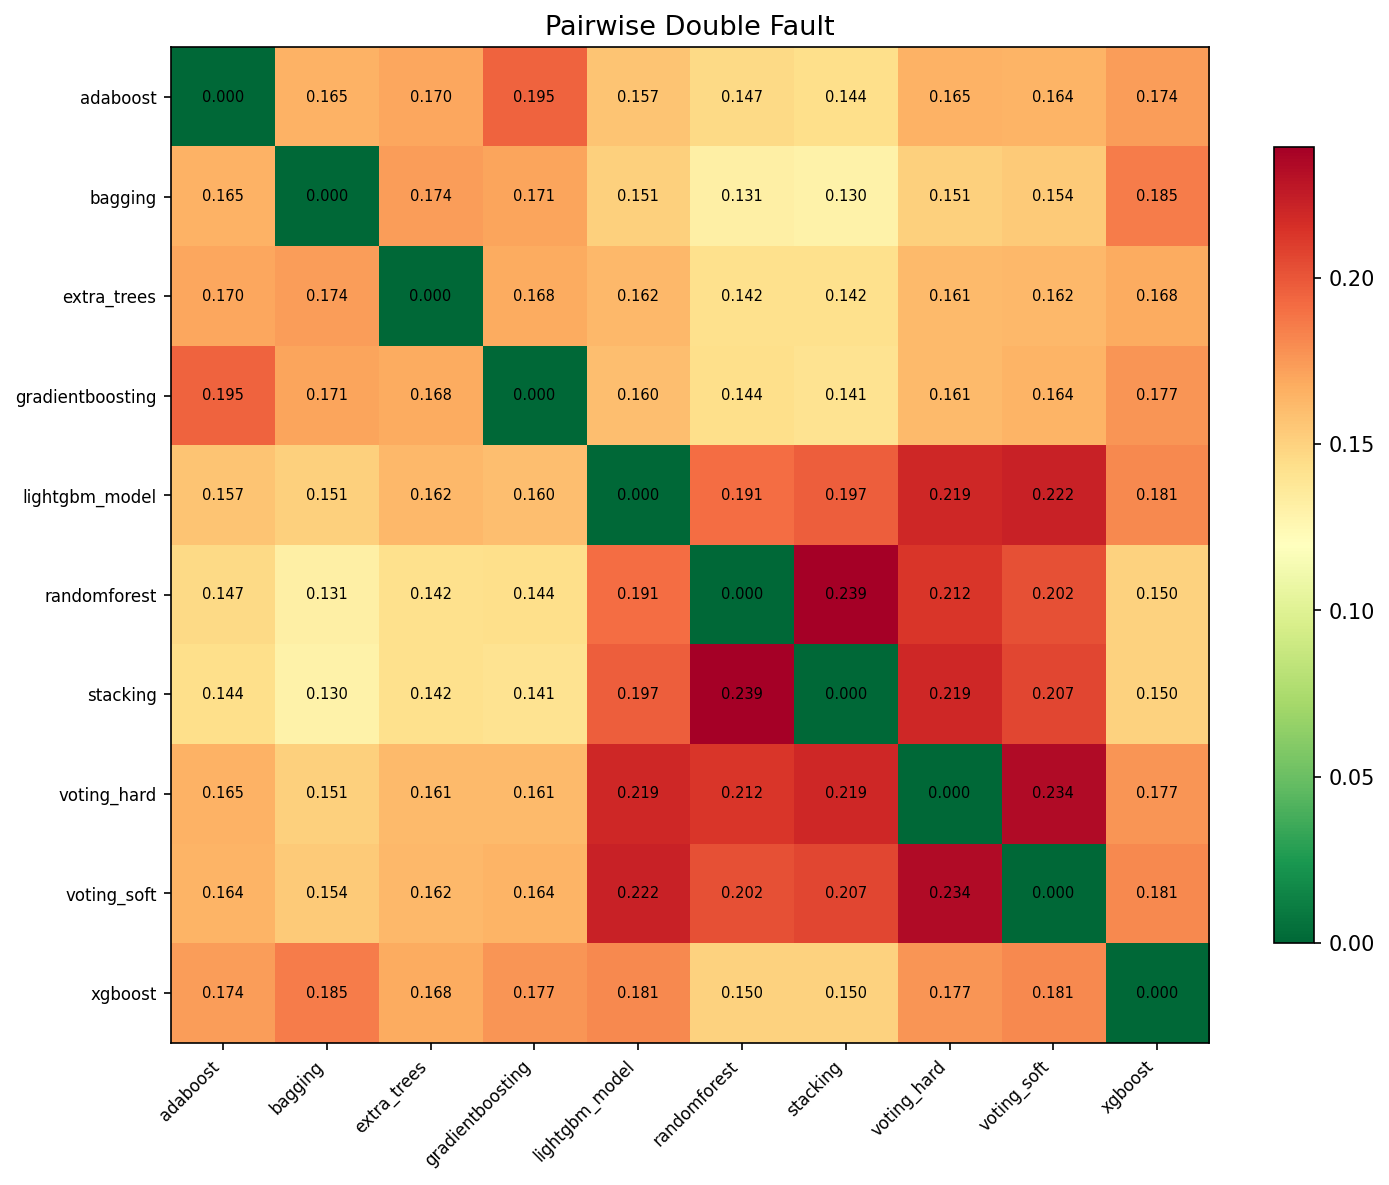
\includegraphics[width=\linewidth]{diversity_double_fault.png}
    {\scriptsize\color{subtletext} Double-fault rate (lower = better)}
  \end{columns}

  \vspace{8pt}
  \centering
  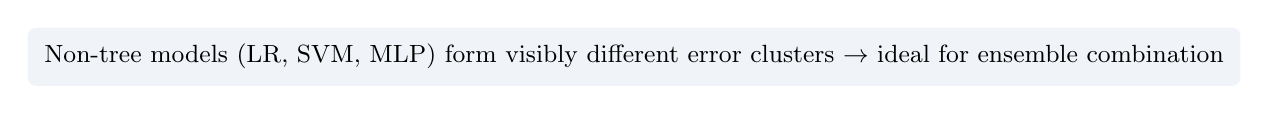
\begin{tikzpicture}
    \node[rounded corners=3pt, fill=softgray, inner sep=6pt, font=\small] {
      Non-tree models (LR, SVM, MLP) form visibly different error clusters $\rightarrow$ ideal for ensemble combination
    };
  \end{tikzpicture}
\end{frame}

% ══════════════════════════════════════════════════════════════
%  5. RESULTS & COMPARISON
% ══════════════════════════════════════════════════════════════
\begin{frame}{Results — All 14 Models}
  \centering
  \begin{adjustbox}{max width=\textwidth}
  \begin{tabular}{lccccc}
    \toprule
    \textbf{Model} & \textbf{F1} & \textbf{Recall} & \textbf{Precision} & \textbf{ROC-AUC} & \textbf{PR-AUC} \\
    \midrule
    \rowcolor{accentteal!12} \textbf{Calibrated Stacking} & \textbf{0.656} & 0.744 & 0.586 & \textbf{0.863} & 0.698 \\
    Random Forest & 0.658 & 0.779 & 0.570 & 0.861 & 0.699 \\
    Stacking & 0.647 & 0.784 & 0.551 & 0.863 & 0.703 \\
    Voting Hard & 0.641 & 0.695 & 0.595 & 0.763 & 0.494 \\
    AdaBoost & 0.639 & 0.744 & 0.560 & 0.845 & 0.638 \\
    Logistic Regression & 0.634 & 0.817 & 0.518 & 0.861 & \textbf{0.708} \\
    SVM & 0.630 & 0.623 & 0.638 & 0.845 & 0.632 \\
    Voting Soft & 0.620 & 0.625 & 0.615 & 0.860 & 0.690 \\
    MLP & 0.603 & 0.550 & 0.667 & 0.861 & 0.702 \\
    Gradient Boosting & 0.611 & 0.534 & 0.715 & 0.858 & 0.687 \\
    \bottomrule
  \end{tabular}
  \end{adjustbox}
  \vspace{4pt}
  {\scriptsize\color{subtletext} Top 10 models shown. Full table includes KNN, Bagging, Extra Trees, XGBoost, LightGBM.}
\end{frame}

\begin{frame}{ROC \& Precision-Recall Curves}
  \begin{columns}[c]
    \column{0.48\textwidth}
    \centering
    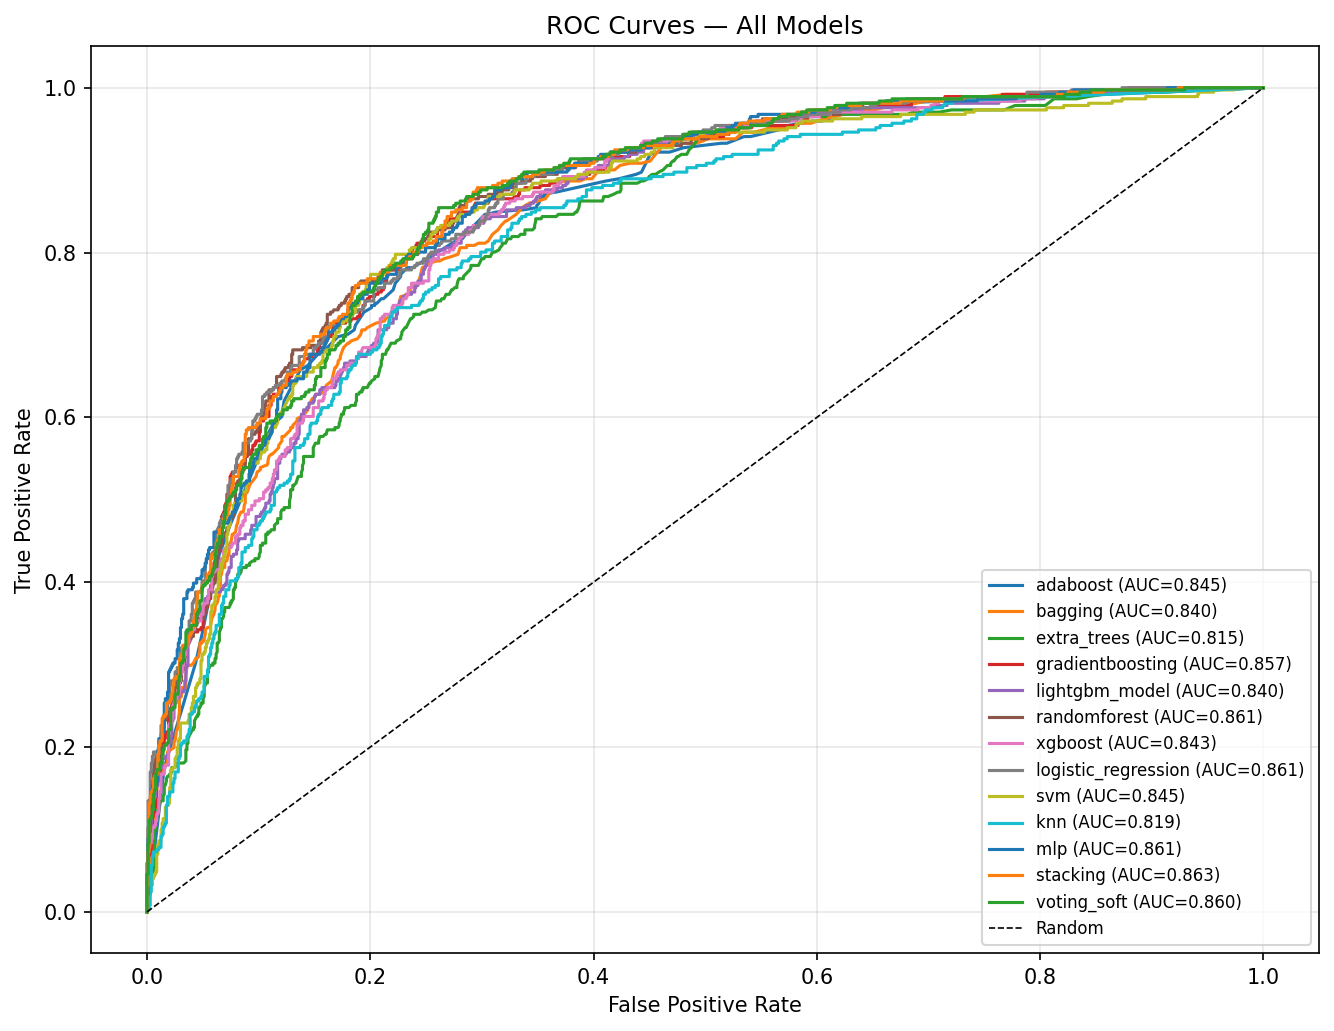
\includegraphics[width=\linewidth]{roc_curves.png}
    {\scriptsize\color{subtletext} ROC Curves — 14 classifiers}

    \column{0.48\textwidth}
    \centering
    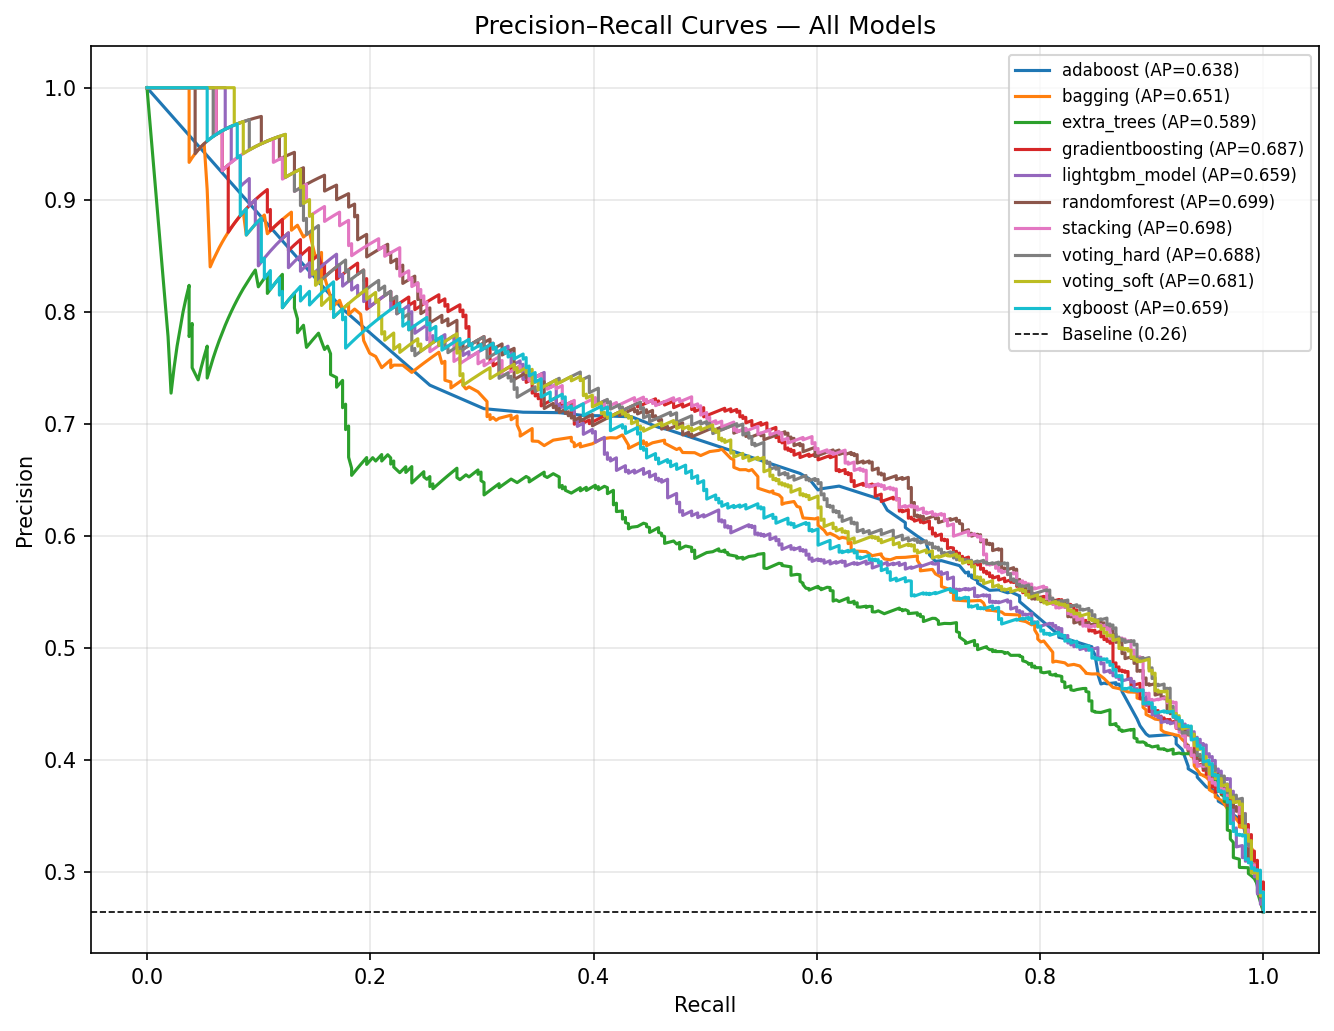
\includegraphics[width=\linewidth]{pr_curves.png}
    {\scriptsize\color{subtletext} Precision-Recall Curves}
  \end{columns}

  \vspace{6pt}
  \centering
  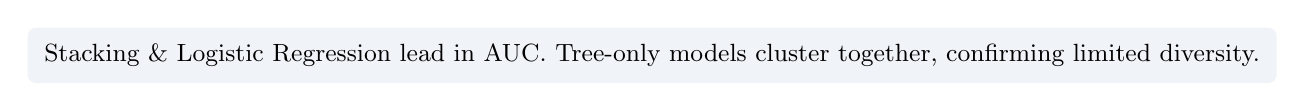
\begin{tikzpicture}
    \node[rounded corners=3pt, fill=softgray, inner sep=6pt, font=\small] {
      Stacking \& Logistic Regression lead in AUC. Tree-only models cluster together, confirming limited diversity.
    };
  \end{tikzpicture}
\end{frame}

% ══════════════════════════════════════════════════════════════
%  6. CALIBRATION & COST OPTIMIZATION
% ══════════════════════════════════════════════════════════════
\begin{frame}{Probability Calibration}
  \begin{columns}[c]
    \column{0.52\textwidth}
    \begin{itemize}
      \item Raw probabilities are often \emphasis{miscalibrated}
      \item Stacking ECE: 0.152 $\rightarrow$ \textbf{0.025} with isotonic {\small\color{successgreen}(6$\times$ better)}
      \item MLP has best native calibration (ECE = 0.014)
    \end{itemize}

    \vspace{6pt}
    \centering
    \begin{adjustbox}{max width=0.95\linewidth}
    \begin{tabular}{lccc}
      \toprule
      \textbf{Model} & \textbf{Original} & \textbf{Platt} & \textbf{Isotonic} \\
      \midrule
      MLP & \textbf{0.014} & 0.051 & 0.040 \\
      Bagging & 0.019 & 0.038 & 0.028 \\
      SVM & 0.023 & 0.035 & 0.031 \\
      Stacking & 0.152 & 0.033 & \textbf{0.025} \\
      Random Forest & 0.124 & 0.039 & 0.041 \\
      \bottomrule
    \end{tabular}
    \end{adjustbox}

    \column{0.46\textwidth}
    \centering
    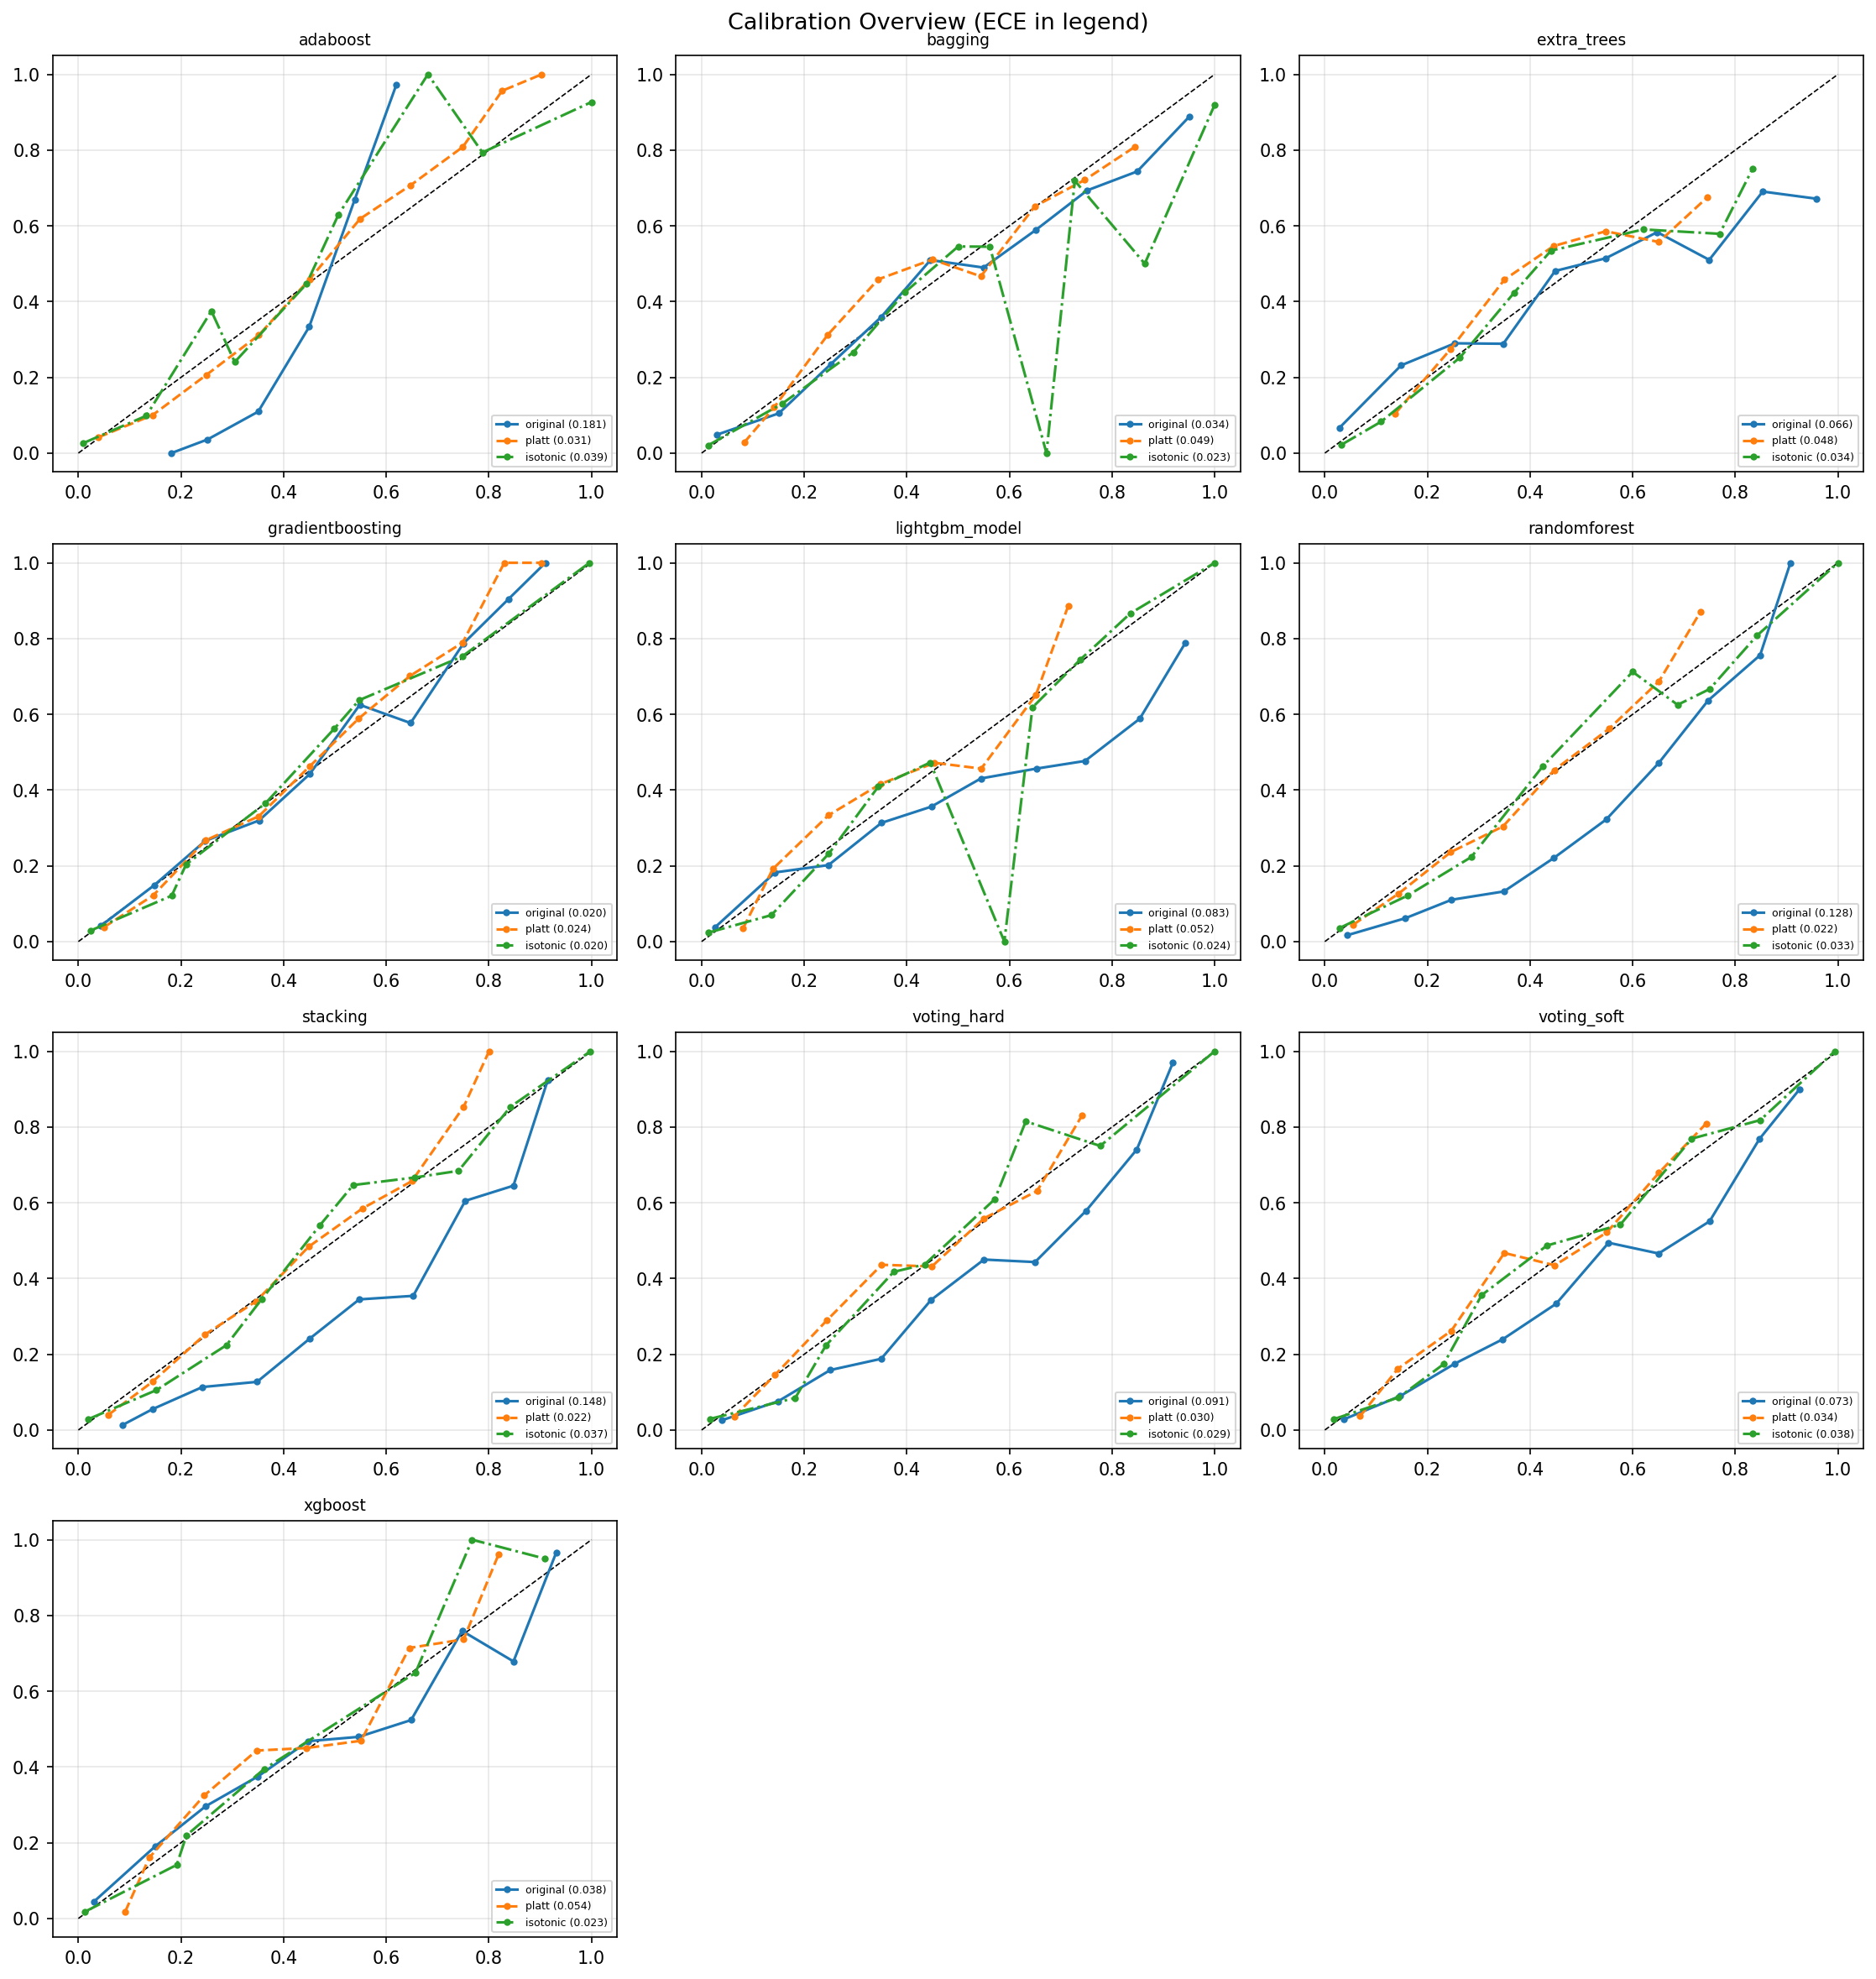
\includegraphics[width=\linewidth]{calibration_overview.png}
    {\scriptsize\color{subtletext} Reliability diagrams — diagonal = perfect}
  \end{columns}
\end{frame}

\begin{frame}{Cost-Sensitive Threshold Optimization}
  \begin{columns}[c]
    \column{0.52\textwidth}
    \begin{itemize}
      \item Default threshold 0.5 is \emphasis{suboptimal for business}
      \item Missing a churner costs \textbf{\$500}, a false alarm costs \textbf{\$50}
      \item Asymmetric costs $\rightarrow$ lower threshold preferred
    \end{itemize}

    \vspace{8pt}
    \centering
    \metricbox{F1-optimal}{$t = 0.397$}
    \hspace{8pt}
    \metricbox{Business-optimal}{$t = 0.14$}
    \hspace{8pt}
    \metricbox{Cost Reduction}{26\%}

    \vspace{8pt}
    \begin{exampleblock}{Impact}
      Moving from $t=0.5$ to cost-optimal threshold saves an estimated \textbf{26\% in business costs} with no model retraining required.
    \end{exampleblock}

    \column{0.46\textwidth}
    \centering
    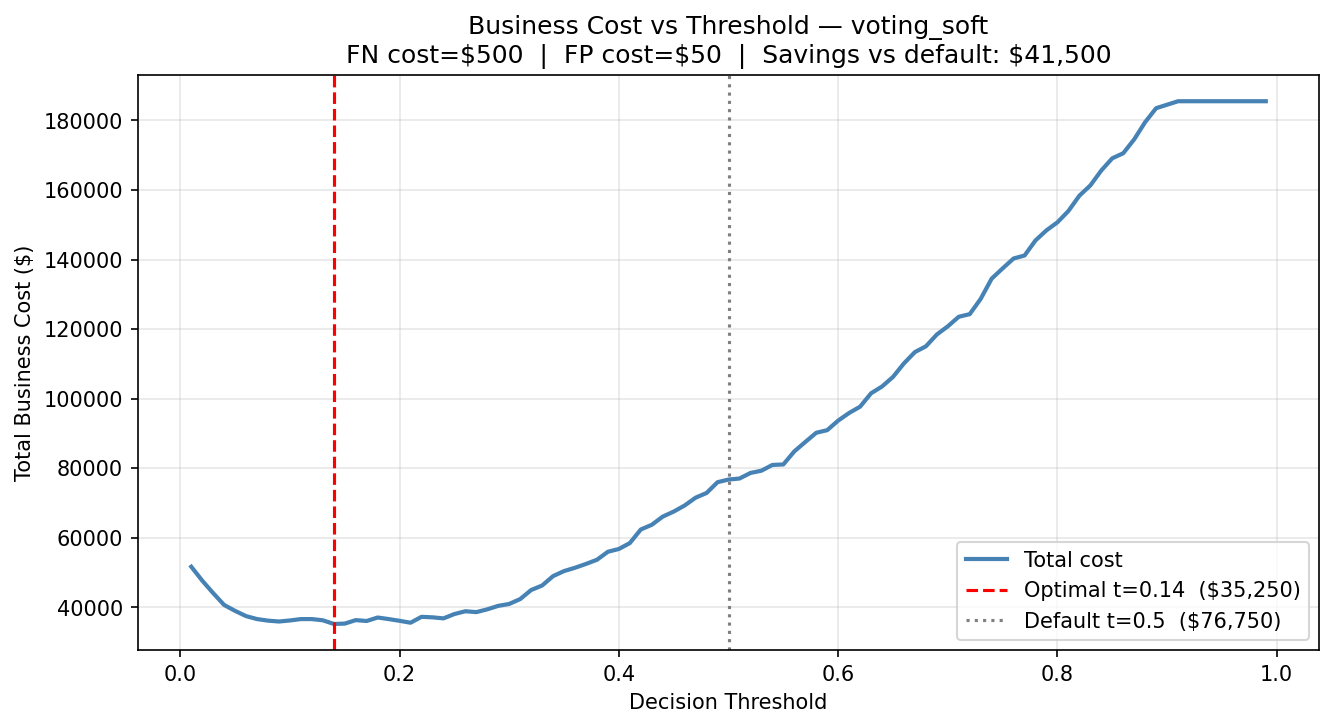
\includegraphics[width=\linewidth]{cost_analysis.png}
    {\scriptsize\color{subtletext} Business cost vs. decision threshold}
  \end{columns}
\end{frame}

% ══════════════════════════════════════════════════════════════
%  7. DYNAMIC ENSEMBLE SELECTION
% ══════════════════════════════════════════════════════════════
\begin{frame}{Dynamic Ensemble Selection (DES)}
  \begin{columns}[c]
    \column{0.55\textwidth}
    \begin{block}{Concept}
      Instead of a fixed ensemble, DES selects \textbf{different classifiers per test instance} based on local competence (k-NN in validation set).
    \end{block}

    \vspace{6pt}
    \centering
    \begin{adjustbox}{max width=0.95\linewidth}
    \begin{tabular}{lcccc}
      \toprule
      \textbf{Method} & \textbf{F1} & \textbf{Recall} & \textbf{AUC} \\
      \midrule
      KNORA-E & 0.615 & 0.615 & 0.721 \\
      KNORA-U & 0.608 & 0.603 & 0.717 \\
      META-DES & 0.601 & 0.580 & 0.710 \\
      DES-KNN & 0.595 & 0.571 & 0.705 \\
      \bottomrule
    \end{tabular}
    \end{adjustbox}

    \column{0.43\textwidth}
    \centering
    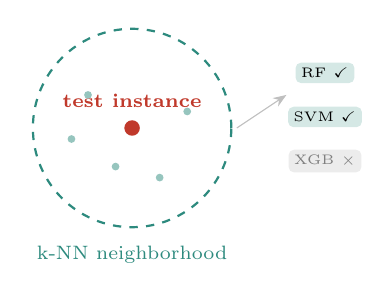
\begin{tikzpicture}[scale=0.7]
      % Test point
      \fill[dangerred] (0,0) circle (4pt) node[above=4pt,font=\scriptsize\bfseries] {test instance};
      % kNN region
      \draw[accentteal, thick, dashed] (0,0) circle (1.8);
      % Neighbors
      \fill[accentteal!50] (-0.8,0.6) circle (2pt);
      \fill[accentteal!50] (0.5,-0.9) circle (2pt);
      \fill[accentteal!50] (-0.3,-0.7) circle (2pt);
      \fill[accentteal!50] (1.0,0.3) circle (2pt);
      \fill[accentteal!50] (-1.1,-0.2) circle (2pt);
      \node[font=\scriptsize,text=accentteal] at (0,-2.3) {k-NN neighborhood};
      % Selected models
      \node[rounded corners=2pt, fill=accentteal!20, font=\tiny, inner sep=2pt] at (3.5,1) {RF \checkmark};
      \node[rounded corners=2pt, fill=accentteal!20, font=\tiny, inner sep=2pt] at (3.5,0.2) {SVM \checkmark};
      \node[rounded corners=2pt, fill=gray!15, font=\tiny, inner sep=2pt, text=gray] at (3.5,-0.6) {XGB $\times$};
      \draw[-{Stealth},gray!50] (1.9,0) -- (2.8,0.6);
    \end{tikzpicture}
  \end{columns}

  \vspace{6pt}
  \centering
  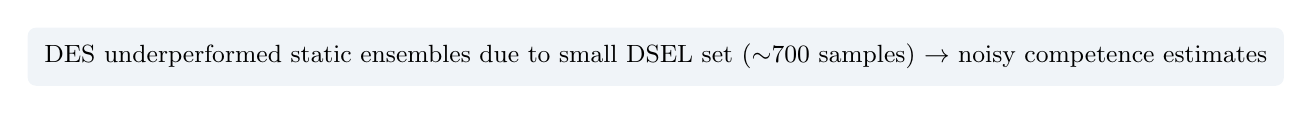
\begin{tikzpicture}
    \node[rounded corners=3pt, fill=softgray, inner sep=6pt, font=\small] {
      DES underperformed static ensembles due to small DSEL set ($\sim$700 samples) $\rightarrow$ noisy competence estimates
    };
  \end{tikzpicture}
\end{frame}

% ══════════════════════════════════════════════════════════════
%  7. WEB PLATFORM
% ══════════════════════════════════════════════════════════════
\begin{frame}{Decision Support Platform — Architecture}
  \centering
  \begin{tikzpicture}[
    box/.style={rounded corners=4pt, minimum width=2.8cm, minimum height=0.9cm, align=center, font=\small\bfseries},
    arr/.style={-{Stealth}, thick, accentteal},
    label/.style={font=\tiny, text=subtletext}
  ]
    % Backend
    \node[box, fill=mainblue!20] (api) at (0,0) {FastAPI\\{\scriptsize 16 endpoints}};
    \node[box, fill=accentteal!15, below=0.3cm of api] (model) {ML Models\\{\scriptsize Joblib artifacts}};

    % Frontend pages - left column
    \node[box, fill=blue!8, minimum width=2.2cm] (exec) at (-5.5,1.5) {\faIcon{tachometer-alt}\ Executive};
    \node[box, fill=blue!8, minimum width=2.2cm] (dash) at (-5.5,0.3) {\faIcon{th-large}\ Dashboard};
    \node[box, fill=blue!8, minimum width=2.2cm] (look) at (-5.5,-0.9) {\faIcon{search}\ Lookup};
    \node[box, fill=blue!8, minimum width=2.2cm] (watch) at (-5.5,-2.1) {\faIcon{eye}\ Watch List};
    \node[box, fill=blue!8, minimum width=2.2cm] (seg) at (-5.5,-3.3) {\faIcon{filter}\ Segments};

    % Frontend pages - right column
    \node[box, fill=orange!8, minimum width=2.2cm] (whatif) at (5.5,1.5) {\faIcon{random}\ What-If};
    \node[box, fill=orange!8, minimum width=2.2cm] (camp) at (5.5,0.3) {\faIcon{bullhorn}\ Campaign};
    \node[box, fill=orange!8, minimum width=2.2cm] (ab) at (5.5,-0.9) {\faIcon{flask}\ A/B Test};
    \node[box, fill=orange!8, minimum width=2.2cm] (rev) at (5.5,-2.1) {\faIcon{dollar-sign}\ Revenue};
    \node[box, fill=orange!8, minimum width=2.2cm] (obs) at (5.5,-3.3) {\faIcon{microscope}\ Observatory};

    % Labels
    \node[label, above=0.1cm of exec] {\textbf{Customer Intelligence}};
    \node[label, above=0.1cm of whatif] {\textbf{Retention Tools}};

    % Connecting arrows
    \foreach \n in {exec,dash,look,watch,seg} {
      \draw[arr, gray!40] (\n.east) -- (api.west |- \n.east);
    }
    \foreach \n in {whatif,camp,ab,rev,obs} {
      \draw[arr, gray!40] (\n.west) -- (api.east |- \n.west);
    }
    \draw[arr] (api) -- (model);

    % Tech labels
    \node[label] at (0,2.2) {\textbf{Next.js 16 + React + shadcn/ui + Recharts}};
    \node[label] at (0,-3.8) {\textbf{Python + scikit-learn + XGBoost + LightGBM + DESlib}};
  \end{tikzpicture}
\end{frame}

\begin{frame}{Platform Features}
  \begin{columns}[T]
    \column{0.48\textwidth}
    \begin{block}{\faIcon{user-shield}\ Customer Intelligence}
      \begin{itemize}
        \item \textbf{Executive Summary} — KPIs, priority actions
        \item \textbf{Portfolio Dashboard} — Risk histogram, tables
        \item \textbf{Customer Lookup} — CRM search, profile, interventions
        \item \textbf{Watch List} — Threshold-filtered risk cards
        \item \textbf{Segment Explorer} — 8-dimension analysis
      \end{itemize}
    \end{block}

    \column{0.48\textwidth}
    \begin{block}{\faIcon{tools}\ Retention \& Analysis Tools}
      \begin{itemize}
        \item \textbf{What-If Simulator} — SHAP-based scenario analysis
        \item \textbf{Campaign Optimizer} — Budget $\rightarrow$ ROI projections
        \item \textbf{A/B Test Simulator} — Strategy comparison
        \item \textbf{Revenue Impact} — Financial risk quantification
        \item \textbf{Model Observatory} — Diversity, calibration, DES
      \end{itemize}
    \end{block}
  \end{columns}

  \vspace{10pt}
  \centering
  {\small\color{subtletext} Screenshots of the platform follow on the next slides $\rightarrow$}
\end{frame}

% ── SCREENSHOT SLIDES ──
% Uncomment these when you have the screenshots
% \begin{frame}{Executive Summary \& Customer Lookup}
%   \begin{columns}[c]
%     \column{0.48\textwidth}
%     \centering
%     \includegraphics[width=\linewidth]{web_executive.png}
%     {\scriptsize Executive Summary}
%     \column{0.48\textwidth}
%     \centering
%     \includegraphics[width=\linewidth]{web_lookup.png}
%     {\scriptsize Customer Lookup}
%   \end{columns}
% \end{frame}
%
% \begin{frame}{Segment Explorer \& Model Observatory}
%   \begin{columns}[c]
%     \column{0.48\textwidth}
%     \centering
%     \includegraphics[width=\linewidth]{web_segments.png}
%     {\scriptsize Segment Explorer}
%     \column{0.48\textwidth}
%     \centering
%     \includegraphics[width=\linewidth]{web_observatory.png}
%     {\scriptsize Model Observatory}
%   \end{columns}
% \end{frame}

% ══════════════════════════════════════════════════════════════
%  8. CONTRIBUTIONS SUMMARY
% ══════════════════════════════════════════════════════════════
\begin{frame}{Contributions}
  \centering
  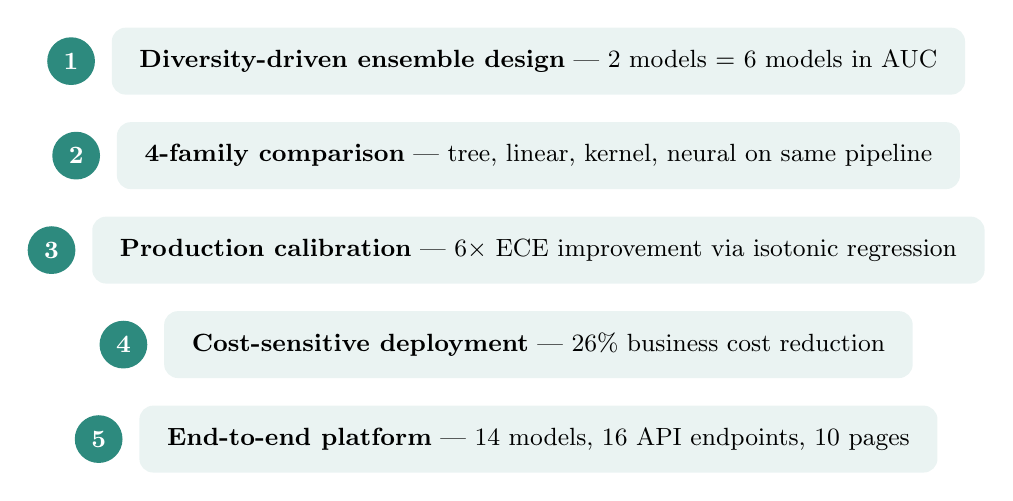
\begin{tikzpicture}[
    contrib/.style={rounded corners=5pt, minimum width=6.5cm, minimum height=0.85cm, align=left, font=\small, inner xsep=10pt},
    num/.style={circle, fill=accentteal, text=white, font=\small\bfseries, minimum size=0.5cm}
  ]
    \node[contrib, fill=accentteal!10] (c1) at (0,3.2) {\textbf{Diversity-driven ensemble design} — 2 models = 6 models in AUC};
    \node[num, left=0.2cm of c1] {1};

    \node[contrib, fill=accentteal!10] (c2) at (0,2.0) {\textbf{4-family comparison} — tree, linear, kernel, neural on same pipeline};
    \node[num, left=0.2cm of c2] {2};

    \node[contrib, fill=accentteal!10] (c3) at (0,0.8) {\textbf{Production calibration} — 6$\times$ ECE improvement via isotonic regression};
    \node[num, left=0.2cm of c3] {3};

    \node[contrib, fill=accentteal!10] (c4) at (0,-0.4) {\textbf{Cost-sensitive deployment} — 26\% business cost reduction};
    \node[num, left=0.2cm of c4] {4};

    \node[contrib, fill=accentteal!10] (c5) at (0,-1.6) {\textbf{End-to-end platform} — 14 models, 16 API endpoints, 10 pages};
    \node[num, left=0.2cm of c5] {5};
  \end{tikzpicture}
\end{frame}

% ══════════════════════════════════════════════════════════════
%  CONCLUSION
% ══════════════════════════════════════════════════════════════
\begin{frame}{Conclusion \& Future Work}
  \begin{columns}[T]
    \column{0.55\textwidth}
    \begin{block}{Conclusion}
      \begin{itemize}
        \item Diversity, not quantity, drives ensemble performance
        \item Calibration is essential for business reliability
        \item Threshold optimization provides immediate cost savings
        \item A complete pipeline from data $\rightarrow$ business decisions
      \end{itemize}
    \end{block}

    \vspace{8pt}
    \centering
    \metricbox{Best F1}{0.656}
    \hspace{4pt}
    \metricbox{Best AUC}{0.863}
    \hspace{4pt}
    \metricbox{Cost Saved}{26\%}

    \column{0.42\textwidth}
    \begin{block}{Future Work}
      \begin{itemize}
        \item Temporal features (usage trends, support history)
        \item SMOTE / ADASYN for class imbalance
        \item Larger DSEL set for better DES performance
        \item Hyperparameter tuning (Optuna)
        \item Real-time prediction API deployment
      \end{itemize}
    \end{block}
  \end{columns}
\end{frame}

% ── THANK YOU ──
\begin{frame}[plain]
  \begin{tikzpicture}[remember picture,overlay]
    \fill[mainblue] (current page.north west) rectangle (current page.south east);
    \fill[accentteal,opacity=0.12] (current page.north west) rectangle (current page.south east);
    \fill[white,opacity=0.03] (11,1) circle (5);
    \fill[white,opacity=0.04] (-1,-2) circle (3);
  \end{tikzpicture}
  \begin{tikzpicture}[remember picture,overlay]
    \node[anchor=center] at (current page.center) {
      \begin{minipage}{0.6\textwidth}
        \centering
        \color{white}
        {\Huge\bfseries Thank You}\\[16pt]
        {\large Questions?}\\[24pt]
        \rule{3cm}{0.3pt}\\[12pt]
        {\small Zaynab Raounak}\\[4pt]
        {\small\color{white!60} April 2025}
      \end{minipage}
    };
  \end{tikzpicture}
\end{frame}

\end{document}
